\section{Evaluation}
\label{eval}

We have used the YFCC100M dataset to evaluate different aspects of our system.
We use the images in the dataset and its associated metadata to implement
an image-search engine based on properties associated to those images.
This is a very common use-case we have encountered when attacking
applications such as smart-retail, sports applications, and video summarization,
where the starting point is a large set of data that must be curated
before proceeding with the data processing and neural network training.
In order to evaluate the different aspects of the performance on the
image search, we built a baseline following the methodology used in the industry, and following what we have done in the past in order to solve
the data search problem, which we describe in Section \ref{images}.

We also cover evaluation we have done using the Video interface VDMS offers,
in order to asses how the implementation performs and scale when used
for video handling.
When it comes to video, ad-hoc solutions have a large number of parameters that
can be tunned, and complex ways to handle the data. Together with that,
there is no system that enables transactional operations over videos files
in the way VDMS does. Because of the two reasons above mentioned,
we focus our efforts in understanding variations in the the performance of
VDMS and its scalability, rather than comparing it to a baseline that
would no represent a fair comparison for either of the systems.
We describe the results in Section \ref{videos}.

Similarly, we explore the behavior of the feature vector functionality in VDMS,
and an evaluation of the different trade-offs that the systems offers for
applications developers. For this, we implemented an image-search application
based on \textit{similarity} search, which we describe in Section \ref{features}


\subsection{YFCC100M Dataset}
\label{dataset}

The Yahoo! Flickr Creative Commons 100m (YFCC100M) dataset is a large
collection of 100 million public Flickr media objects created to provide free,
sharable multimedia data for research. This dataset contains approximately
99.2 million images and 0.8 million videos with metadata characterized by
25 fields such as the unique identifier, userid,
date the media was taken/uploaded, location in longitude/latitude coordinates,
device type the media was captured, URL to download the media object,
and the Creative Commons license type information.
The YFCC100M dataset also used a deep learning approach to generate autotags
which is a set of comma-separated concepts such as people, scenery, objects,
and animals and confidence scores generated from 1,570 trained
Caffe classifiers ~\cite{Thomee_2016}. Together with the autotag, there is a
probability associated to each tag to indicate the certainty level of the tag
in that image/frame.
We have also used feature vectors generated for every image and first frame
of every video \cite{features} to implement similarity search.
Given that there is no standard benchmark oriented towards visual data queries,
we have built a series of queries to filter this dataset that is model after
our internal use cases for many of the mentioned applications we have worked
with.


\subsection{Experimental Setup}

As a baseline, and given that there are no other open-source system
that implements similar functionality and interfaces as VDMS,
we implemented an equivalent visual data management system comprised of a
combination of widely available, off-the-shelve components:
MySQL Server 5.7 (for storing metadata),
Apache Web Server 2.4.18 (as interface for image access), and
OpenCV 3.3 (to provide pre-processing operations on images).
We have implemented a set of client-side applications that takes care
of retrieving the components from the different systems, and applies
pre-processing operations when needed.
For visual data workloads, building an approach like the one
implemented as a baseline for this work
is the common practice in the industry \cite{heystack, tao}.

For all our experiments, we use 2 servers, one hosting a VDMS server and
another hosting a the Baseline implementation.
Both servers have a dual-socket Intel\textsuperscript{\textregistered}
Xeon\textsuperscript{\textregistered} Platinum 8180 CPU @ 2.50GHz (Skylake),
each CPU with 28 physical cores with multithreading enabled,
for a total of 112 logical cores per server.
The server hosting MySQL has 256GB of DDR4 DRAM, while the server hosting VDMS
has 64GB of DDR4 DRAM. Both servers run Ubuntu 16.04.
The client application (running the queries and measuring round-trip time)
is connected to the server through a 1GB wired link through
a 10GB-backplane switch.

Figure~\ref{fig:systems} shows a logical view of the difference between the
interaction of the client application (which wants to retrieve metadata and
imaged) with VDMS (left) and the baseline (right).
The client application was implemented using Python 3 for both VDMS and
the baseline.

It is worth noting that the images are stored in a shared repository
(ext4 filesystem on a RAID 6 configuration of 16TB) that both Apache WebServer
and VDMS have direct access. In the case of the baseline, metadata is
stored in MySQL using an attached SSD disk.
Even if VDMS has native support for Optane Persistent Memory,
we do not use it in this experiment because of fairness of comparison w.r.t
MySQL (which was not design for Persistent Memory type of storage).
The benefits of Persistent Memory on metadata operations is left
for another paper, and outside the scope of this evaluation.
For this experiment then, in the case of VDMS we simply use a similar
attached SSD disk to store metadata.
Even if PMGD, the graph database used by VDMS, is designed for PM,
it can deliver good performance when using SSDs directly.

\begin{figure*}[]
\centering
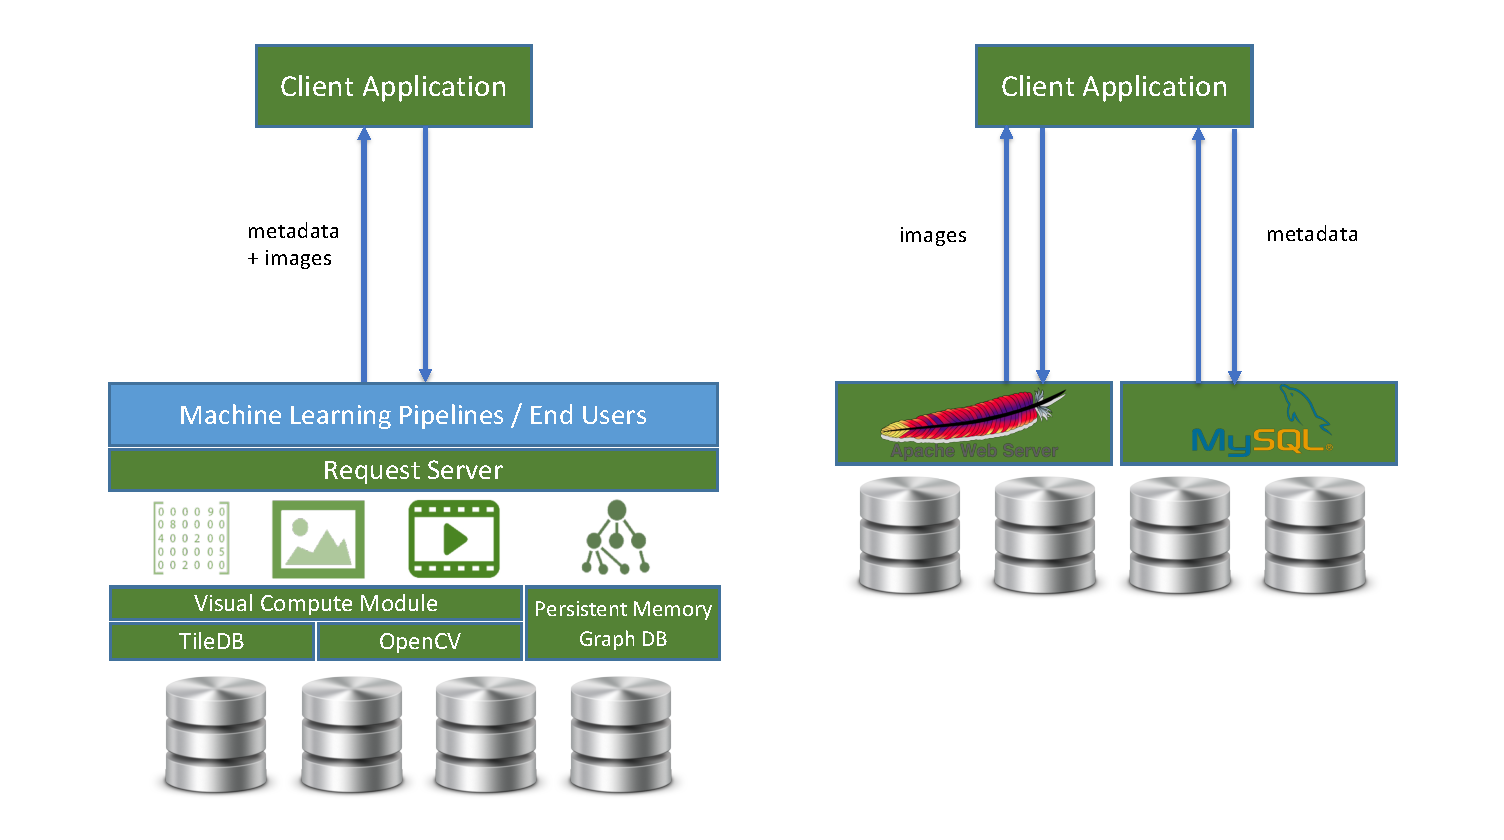
\includegraphics[width=\textwidth]{figures/comparison_system}
\caption{Comparison Systems}
\label{fig:systems}
\end{figure*}

For the metadata, we built VDMS and MySQL databases
using the YFCC100M dataset with incremental database sizes.
For simplicity, we named the database based on the approximate number of images
it contains, as follows: 100k, 500k, 1M, 5M, 10M, 50M, 100M.
The exact number of images/elements on each database is shown in
Table~\ref{table:vdmsnodes} and ~\ref{table:mysqltables}
For each database size, we created an instance of VDMS using YFCC100m metadata,
the YFCC100m machine-generated \textit{autotags} associated with
each metadata identifier, and the list of 1,570 \textit{autotags}
using 100 concurrent VDMS Python clients.
Internally, that information is represented as a property graph,
where we have one node for each image, one node for each tag
(always 1570 tags), and connections between images.
For instance, if an image has 4 \textit{autotags} assigned,
there will be 4 connections between that image and
the different nodes for those \textit{autotags}.
The information about the probability the \textit{autotag} present in an image
is expressed as a property in the \textit{connection} between the 2 nodes.
Figure \ref{fig:graph_representation} shows an example on two images and
2 \textit{autotags}, and the \textit{connections} between those \textit{autotags}
and the images.
Image id: 23143252 has two \textit{autotags} assigned:
\textit{Alligator} with probability 0.285 and \textit{Lake} with probability 0.872.
Image id: 86756231, on the other hand, has a single \textit{autotags} assigned:
\textit{Alligator} with probability 0.894.

\begin{figure}[]
\centering
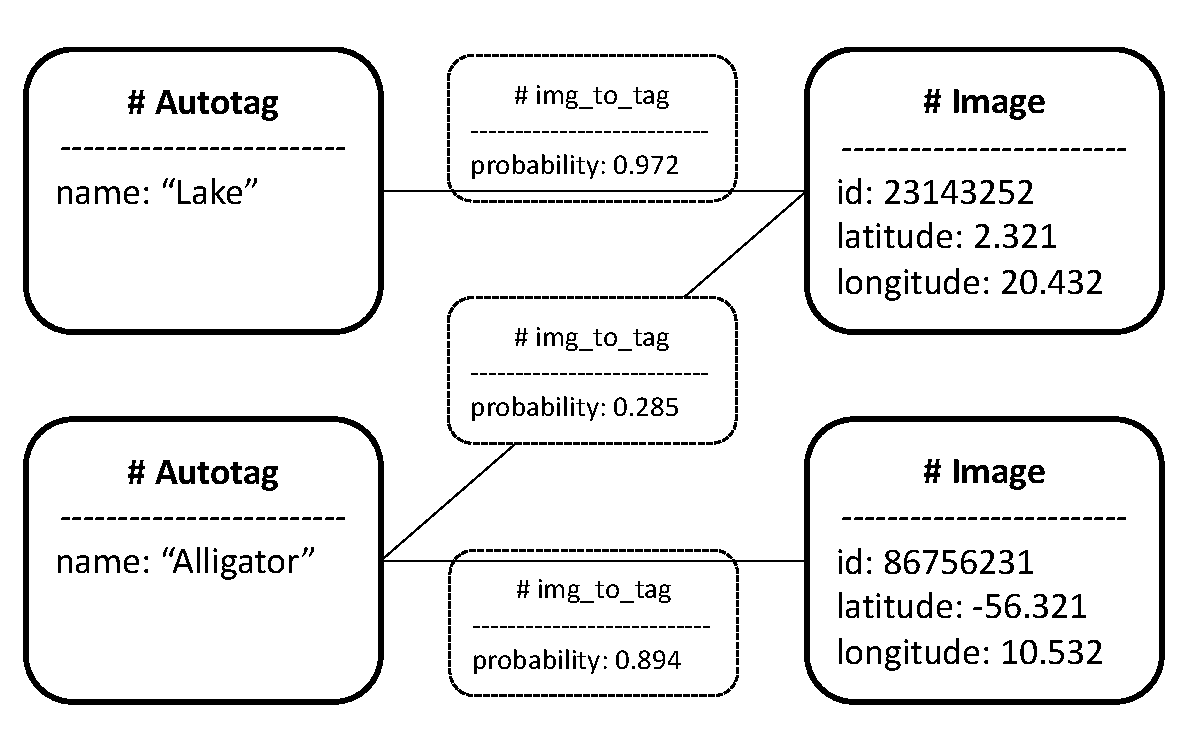
\includegraphics[width=\columnwidth]{figures/graph_representation}
\caption{VDMS Data Representation Using a Property Graph:
Example on two images and 2 \textit{autotags} with
their respective probabilities expressed in the \textit{connection}.
Image id: 23143252 has two \textit{autotags} assigned:
\textit{Alligator} with probability 0.285 and \textit{Lake} with probability 0.872.
Similarly, Image id: 86756231 has a single \textit{autotags} assigned:
\textit{Alligator} with probability 0.894.}
\label{fig:graph_representation}
\end{figure}

Because there are on average 8 tags assigned to each image,
there will be around 8 times more connections than images, as can be seen
in Table~\ref{table:vdmsnodes}.
Also, each image node will contain multiple properties associated
with that object.
Using the Python Client Module, we insert 1,570 nodes for the \textit{autotags},
and then insert nodes for the YFCC media objects (images or videos)
with the associated metadata.
Adding the autotag confidence scores is a recursive process and requires more
complex queries than adding the previous nodes.
For each metadata identifier in \textit{autotags},
the query must find the associated metadata node and tag node.
A connection between the two nodes is created with the confidence score as a
property. The number of metadata nodes are dependent on the database size and
the connections are responsible for 90\% of the elements in each database as
shown in Table~\ref{table:vdmsnodes}.
It is important to note that the metadata identifier, \textit{autotags}, and
longitude/latitude coordinates are set as indexes of the database to allow
faster retrieval of the metadata.

\begin{table}[h]
\caption{VDMS Database - Number of Elements}
\centering
\begin{tabular}{c c c c}
\hline\hline
DB Name & \# Images & \# Connections & \# Autotags\\
\hline
100k & 100,000     & 848,432      & 1,570\\
500k & 500,000     & 4,249,500    & 1,570\\
1M   & 1,000,000   & 8,503,045    & 1,570\\
5M   & 5,000,000   & 42,505,478   & 1,570\\
10M  & 10,000,000  & 85,040,404   & 1,570\\
50M  & 50,000,000  & 425,162,070  & 1,570\\
100M & 99,205,984  & 895,572,430  & 1,570\\
\hline
\end{tabular}
\label{table:vdmsnodes}
\end{table}

Each MySQL database is created in a similar manner but the data is represented
as three tables, following the relational model:
1) \textit{images} table, contains one row per image,
and a column for each property
associated with the images (some of which are listed in \ref{dataset});
2) \textit{taglist} table: contains one row per each autotag elements
(always 1570 rows);
3) \textit{autotags} table: contains on row per each autotag
assigned to an image, each row containing a foreign key to the
image and a foreign key to the tag, and
the probability assigned to that tag belonging to that image.
Given that there are 8 autotags, on average, per image, the \textit{autotags}
table has around 8 times the number of rows present in the
\textit{metadata} table, as can be seen in~\ref{table:mysqltables}.

THIS NEEDS FIX, NOT SURE I UNDERSTAND WHAT YOU MEAN:
By default, MySQL uses infinite number of threads inside InnoDB when processing
requests using four threads per IO read/write.
In some cases, when creating large databases data locks may occur to protect the
data from concurrent updates.
To minimize locking in our runs, we increased the InnoDB buffer pool size to
increase the amount of memory allocated to in-memory data structures
~\cite{mysql,mysql_blog}.

Using a Python client and simple queries, the \textit{taglist}
table is read from the list of tags with an auto-incremented
\textit{tagid} as a primary key and the metadata table
is read from the YFCC100m metadata using the identifier as a primary key.
The \textit{autotags} table contains the generated autotags and
probabilities for entries of the \textit{images} table.

To generate the table, we split the \textit{autotags} data for each database
by the image identifier and autotag into new files.
The new files are read into the \textit{autotags} table with the image
identifier and \textit{tagid} as foreign keys.

\begin{table}[h]
\caption{MySQL Database - Number of Rows in each Table}
\centering
\begin{tabular}{c c c c}
\hline\hline
 & \multicolumn{3}{c}{Table}\\
\cline{2-4}
DB Name & images & autotags & taglist\\
\hline
100k & 100,000    & 848,912     & 1,570\\
500k & 498,707    & 4,241,200   & 1,570\\
1M   & 1,000,000  & 8,508,380   & 1,570\\
5M   & 4,987,379  & 42,425,905  & 1,570\\
10M  & 10,000,000 & 85,095,265  & 1,570\\
50M  & 50,000,000 & 425,446,208 & 1,570\\
100M & 99,206,564 & 896,002,496 & 1,570\\
\hline
\end{tabular}
\label{table:mysqltables}
\end{table}

\begin{figure}[]
\centering
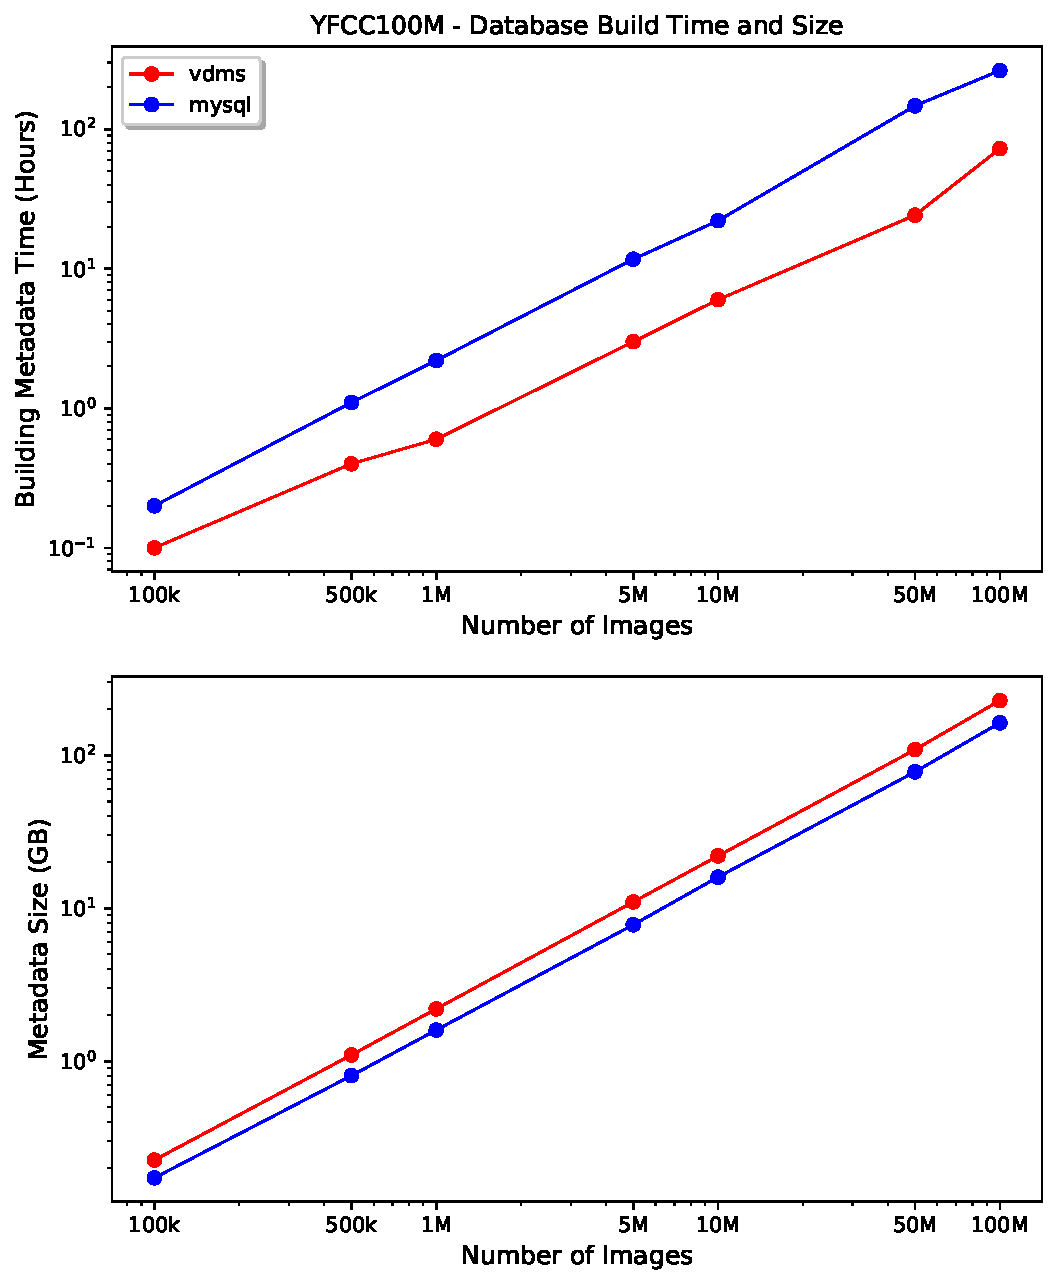
\includegraphics[width=\columnwidth]{figures/db_time_size}
\caption{Time (in hours) to build and size (in GB) of MySQL and VDMS databases}
\label{fig:db_time_size}
\end{figure}

The VDMS and MySQL databases have comparable number of elements as shown in
Table~\ref{table:vdmsnodes} and ~\ref{table:mysqltables}, and the differences
can be attributed to failures in data preparation/loading because of
incomplete/inconsistent formating, which is common on large datasets.
The difference is less than 0.1\% in terms of number of elements (images and/or
metadata information).

\subsubsection{Database Loading Time}

One of the first things we noticed is the difference is loading times,
where VDMS outperforms MySQL by a large margin.
Figure~\ref{fig:db_time_size} illustrates how VDMS can build databases
faster than MySQL, and how the speedup is sustained as the database size grows.
Key difference in the build times are attributed to the low-level
implementation of how MySQL reads and stores data from the files and the
optimizations (increased InnoDB pool size, etc.) needed
to handle large datasets such as YFCC100m.
On average, it took MySQL 3.72x longer to build each database than VDMS.
For example, to build the 100M database, MySQL took 263 hours
while VDMS only needed 72.5 hours.

\subsubsection{Database Storage Footprint}

Another aspect important to note is that
VDMS requires more storage for metadata, shown in Figure~\ref{fig:db_time_size}.
This is space used to store information about each node/connection.
The Graph Database internal to VDMS (called PMGD) was designed for performance,
specially in environments where persistent memory is present.
This design decision comes as a trade-off for storage footprint, which is
noticeable in our results.
VDMS required 30-41\% more storage than MySQL for storing the same amount
of metadata.
This may become a factor if storage is a limitation, but it should also be noted
that even if we have a 41\% increase in metadata size,
metadata accounts for less than 2\% of the overall database size.
Take, for example, the largest database (both metadata and images) we built
(100M): around 230GB of metadata and 12TB of images.
On the other hand, in systems were persistent memory is a scarce resource,
the increase storage foot print of PMGD may represent a challenge.

%=========================================

\subsection{Images + Metadata}
\label{images}

In order to evaluate VDMS and the baseline on our use-case queries,
we implemented 4 queries that that filter and retrieve certain specific images.
We choose these queries because they represent typical use-case where a
cohort of images is to be retrieve and processed from a large corpus of data.
As we mentioned before, we took this approach due to the lack of a standard
benchmarks that are oriented towards visual data retrieval.
We use the metadata associated to the images to filter said images.
In particular, this dataset contains a set of 1570 machine generated
tags (\textit{autotags})assigned to the images depending on the content.
\textit{autotags} includes things like objects (chair, person, people, etc), and
concepts like places (indoor, outdoor, lake) and others (party, etc).
Together with each \textit{autotag}, a probability is assign.
This is, an image can have the \textit{autotags} people, person, party,
outdoor, and each \textit{autotag} assigned will be accompanied by a
probability of that \textit{autotags} being present in that image.
As mentioned earlier, there are 8 tags assigned to each image on average.
Also, some images have geo-location information (latitude/longitude).

We use the \textit{autotags} (as they contain information about
the content of the image), as well as the geo-location
(as an example of properties of the images used used for search and filtering).

On top of that and for our use case, we would like to extract more information
about the content of the image through the use of ML,
such as Convolutional Neural Networks TODO-CITE HERE.
For this, we resize the images to 224x224, which is the input layer size for
a popular neural network for object detection on images: ResNet TODO-CITEHERE.

To evaluate the access to metadata and images,
we use the following four queries, modeled after our internal use cases:
\begin{enumerate}
\item {\bf {\em 1tag}}: Find metadata/images with 1 specific autotag (i.e. alligator, lake, etc).
\item {\bf {\em 1tag\_resize}}: Find metadata/images with 1 specific autotag and resize to 224x224.
\item {\bf {\em 1tag\_resize\_geo}}: Find metadata/images with 1 specific autotag, resize to 224x224, and in a particular geolocation (with a 20 degrees radius in latitude and longitude).
\item {\bf {\em 2tag\_resize\_geo}}: Find metadata/images with 2 specific tags (i.e. alligator AND lake) and resize to 224x224.
\end{enumerate}

It is important to note that when querying for images with certain
\textit{autotags}, we also apply a filter using the probability.
For instance, we only retrieve images with a autotag \textit{alligator}
and a probability higher than 92\%.
This probabilities are both present in VDMS (in the form of a property
of the \textit{connection} between the image and that \textit{autotag}),
as well as in MySQL (in the form of a column in the \textit{autotags} table
that links images with tags.

\begin{figure}[]
\centering
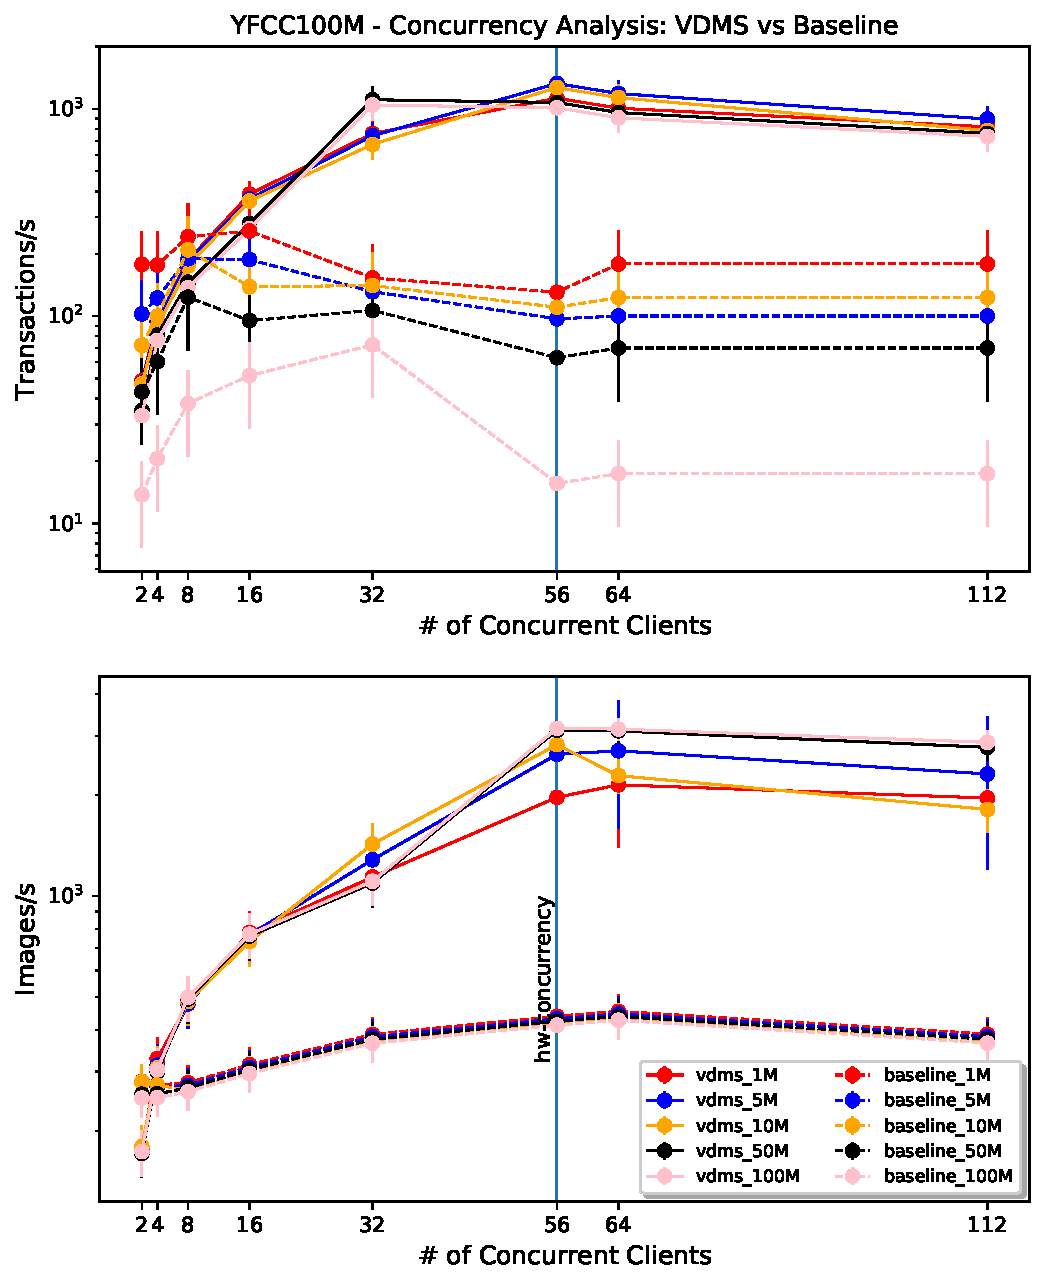
\includegraphics[width=\columnwidth]{figures/concurrency_comparison}
\caption{Concurrency Analysis on Query \textit{1tag\_resize} \- VDMS vs Baseline}
\label{fig:concurrency_comparison}
\end{figure}

% We decided to remove this image because it is redudant with the concurrency
% analysis.
% \begin{figure}[t!]
% \centering
% 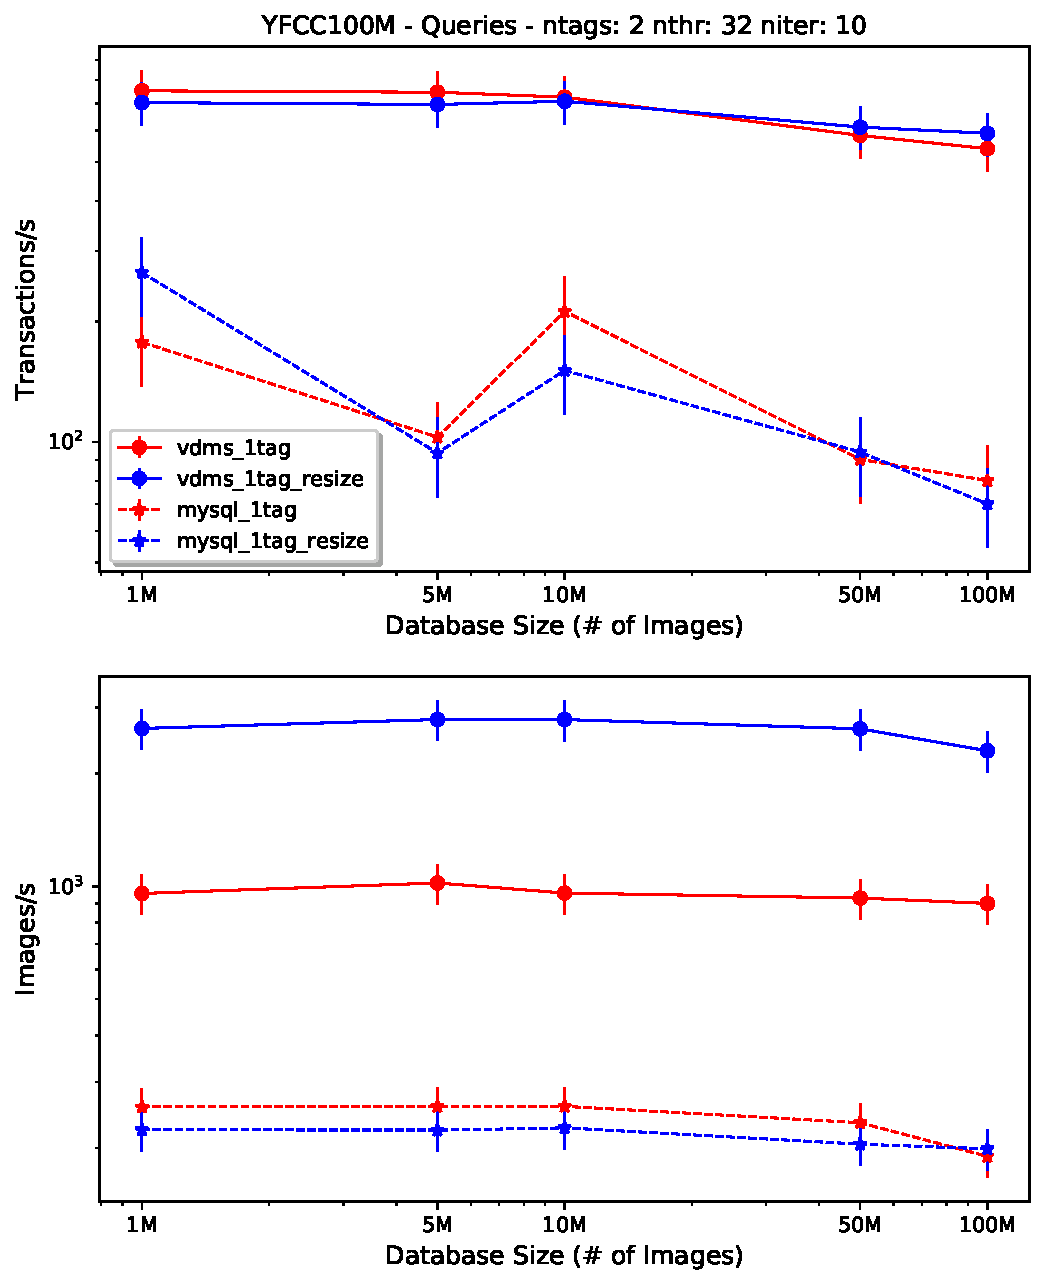
\includegraphics[width=\columnwidth]{figures/queries_throughput_32}
% \caption{Queries - Throughput - 32 Clients}
% \label{fig:q_throughput_32}
% \end{figure}

\begin{figure}[t!]
\centering
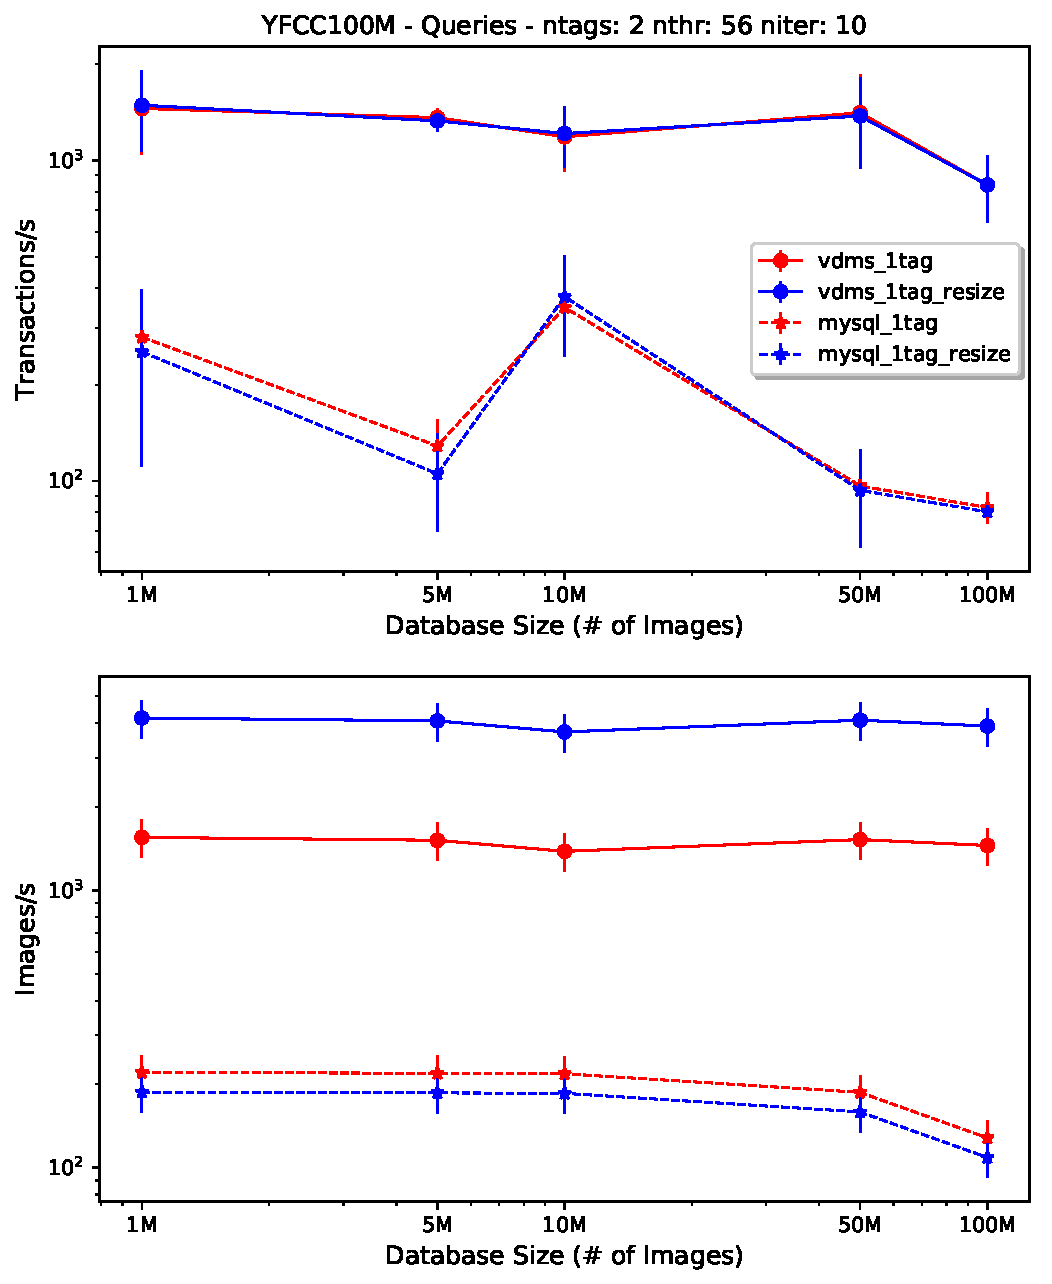
\includegraphics[width=\columnwidth]{figures/queries_throughput_56}
\caption{Queries - Throughput - 56 Clients}
\label{fig:q_throughput_56}
\end{figure}

Image search based on metadata is very expensive on large databases.
Because of the large volume of data, the processing of the retrieve images
is perform in parallel, using multi-core and/or distributed systems.
For instance, a common implementation of an image processing pipeline
would involve the use of distributed processing frameworks
like Hadoop \cite{hadoop} or Spark \cite{spark}.
Consequently, it is key that the data management system used supports
concurrency, providing multiple workers with data in parallel.
The ability to scale with the number of simultaneous clients is key for the
applicability of visual data management systems like VDMS.

Figure~\ref{fig:concurrency_comparison} illustrates a concurrency analysis for
the \textit{1tag\_resize} query, described above, using both VDMS and
the baseline to evaluate the scalability of both solutions, as the
size of the databases grows and as the number of concurrent clients grows.

It is important to note that the size of the result (number of images retrieved)
is linear with the size of the database. This is, if a query returns 100 images
for the 1M database, it will return around 1000 images for the 10M database.
This poses a problem when evaluating performance as database increase,
and clearly understanding the measurements.
Because of this reason, we control the number of returned images for all the
database using the probability of the \textit{autotags}, so that the queries
in this experiment returns a similar number of images for all database sizes.
Essentially, as the size of the database increase, we increase the probability
threshold for the queries. We do this for both VDMS and the baseline, of course.

The first thing to notice is that when it comes to retrieving metadata
in the case of VDMS, (Figure ~\ref{fig:concurrency_comparison} (top),
the size of the database (in terms of number of images) does not have
a strong effect on the performance
(measured in aggregated transactions per second).
This means that even as database increase in size, there is no large increase
in the query time.



 the number of concurrent clients to use for the per-query performance analysis.
This figure shows the metadata performance plateaus at 32 clients and
the image performance at 56 clients for a simple query.
% To further investigate, Figure~\ref{fig:q_throughput_32} and
% Figure~\ref{fig:q_throughput_56} illustrate the throughput performance
% for the \textit{1tag} and \textit{1tag\_resize} queries for 32 and 56 clients,
% respectively.
On the 56-client experiment, a 10x difference can be seen between VDMS and
baseline in metadata throughput while 32 clients is similar but not as high.
The overall performance for both MySQL and VDMS is better with 56 clients;
therefore, we used this value for our per-query analysis.

\begin{figure}[]
\centering
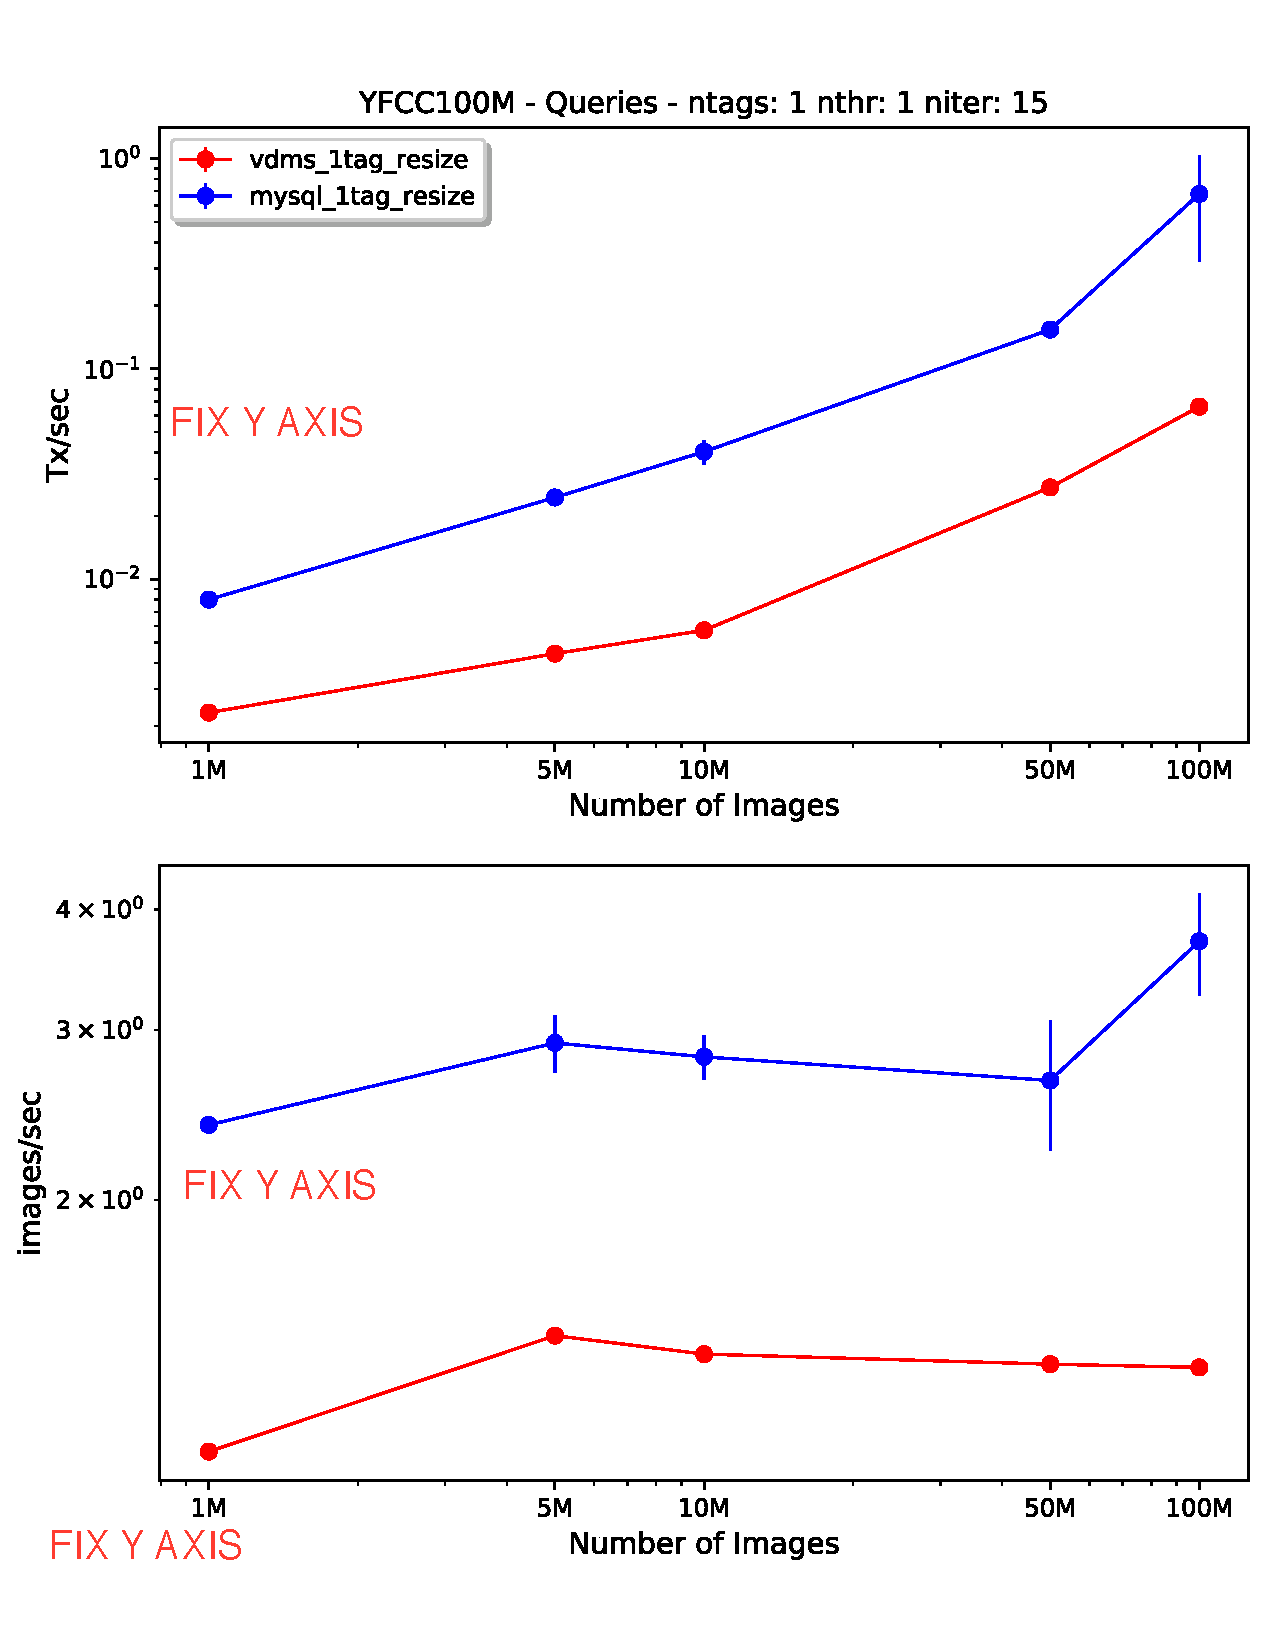
\includegraphics[width=\columnwidth]{figures/q1_latency}
\caption{Query 1 - Latency}
\label{fig:q1_latency}
\end{figure}


%=========================================

\subsection{Videos}
\label{videos}

VDMS provides full support for video storage and operations.
This includes support for encoding/decoding and trans-coding of
\textit{mp4}, \textit{avi}, and \textit{mov} containers,
as well as support for \textit{xvid}, \textit{H.263} and \textit{H.264} encoders.
This is supported through the Visual Compute Module that provides an abstraction
layer on top of OpenCV (and \textit{ffmpeg} directly).
All the operations supported for images in VDMS are also supported at the
video and frame level on the API. On top of that, there are a number of
video-specific operations that are supported, such as the interval operations,
that allow users to retrieve clips at different
frames-per-second (FPS) versions of the video.

All this functionality is provided and integrated with the rest of the
metadata API as part of the comprehensive VDMS interface. This makes it
possible for users to interact with metadata and video in a transactional
manner, enabling users to run queries like: "Retrieve all the videos
where there is a lake with probability higher than X, converting all videos
to \textit{H.264} \textit{mp4} of size 224x244".
In particular, this functionality was used internally to select a subset
of videos with the right licenses for a video summarization application.

To the best of our knowledge, there is no solution that can provide
all the functionality mentioned above. Also, implementing a baseline is a very
complex task as there is a large number of options and parameters that can
be chosen, which makes it hard to accurately compare against VDMS functionality.
For this reason, we chose to make a study using VDMS in various scenarios,
and analysis what is the impact of having the overhead of VDMS' Request
Server in the overall access time.

\begin{figure*}[ht!]
\centering
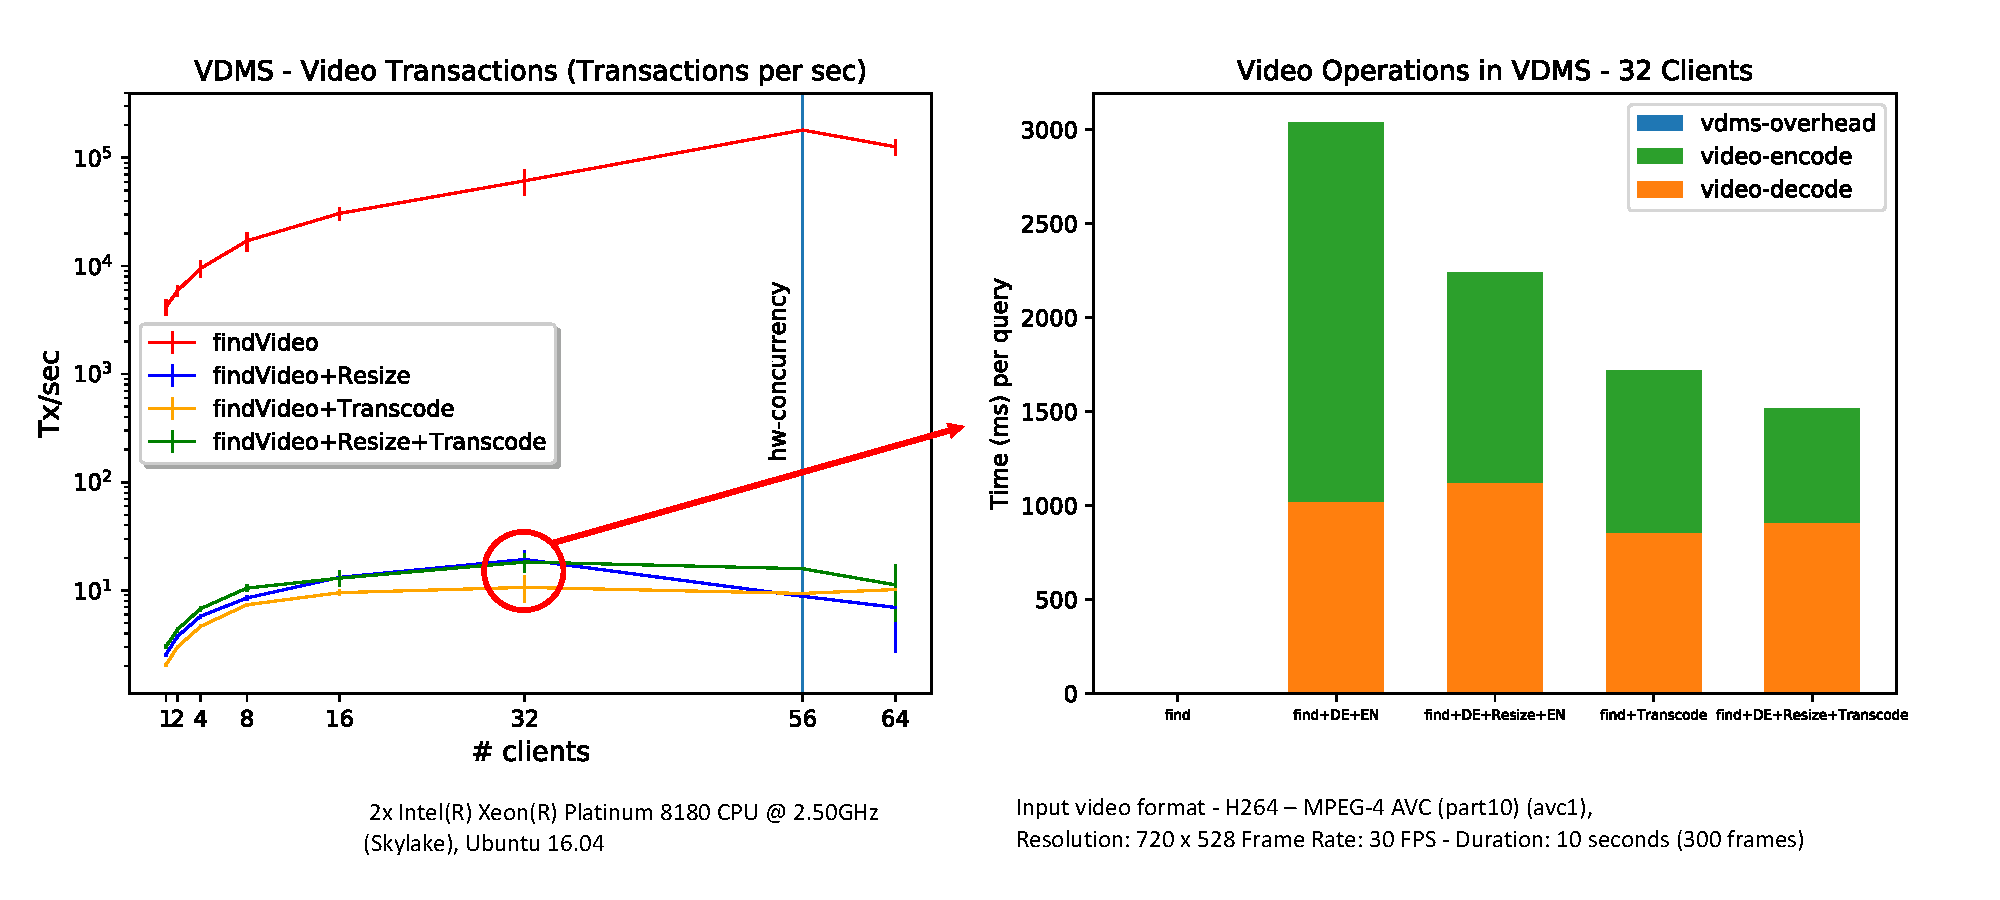
\includegraphics[width=\textwidth]{figures/video_overhead}
\caption{Concurrency (left) and Overhead (right)}
\label{fig:video}
\end{figure*}

Figure \ref{fig:video} shows the analysis of different queries aimed to retrieve
a video using VDMS interface. We show how VDMS increases throughput of serving
a video object as the number of simultaneous client increases, as well as the
overhead VDMS introduces in the overall query execution time.
The figure on the left compares the number of video transaction per second
(i.e., number of videos returned per second) when different operations
are executed as part of the transaction. The upper-bound of this would be
simply returning the video as-is (without running any encoding/decoding or
operation), represented by the red line. This query is the upper-limit because
it essentially translates to reading the video from the file-system and sending
it over a TCP/IP socket, without any other overhead or operations.

We also run a set of other queries that involve: (a) running a resize operation
on the video and, consequently, needs a decoding and
encoding operations as well (blue line),
(b) transcoding, meaning the use a different container and encoder
than the one originally used (yellow line), and (c) both resize and transcoding.
Note that the resize operation performs a downsize, which translates in less
data being sent over the wire. This is specially noticeable when supporting 32
simultaneous clients, where the systems provides more videos per second due to
sending less data to the client, when compares to just transcoding and not resizing (yellow line).

We can see that the system performs best when using all the physical cores.
COMPLETE THIS BETTER.

WE SHOULD ADD HERE SAMPLES OF THE QUERYS TO SHOW HOW THESE ARE RETRIEVED.

Because we see almost 3 orders of magnitude drop in performance when including
operations as part of the query, we wanted to understand where most of the time
was spent on the query, and optimize the Request Server and Visual Compute Module
if necessary. For this, we run the experiment shown at
Figure \ref{fig:video} (right) which breaks down the different components of the
queries. This figure shows that more than 97\% of the query execution is spent
on encoding/decoding operations, which is well-known to be a
heavy and compute intensive operation.
On the one hand, this results show that VDMS introduced overhead for
video operation is minimal. On the other hand, this result means a
limit on the opportunities for optimization for video queries given
that biggest time factors are accounted by encoding/decoding, which is
outside the scope of VDMS.
This result also was the inspiration point for one optimization we included
in future versions of VDMS, which involves using \textit{ffmpeg} C++ API to
limit the number of frames being encoding/decoding when possible.

%=========================================

\subsection{Feature Vectors}
\label{features}

Another key differentiating factor of VDMS is that it allows the creation of
indexes for high-dimensional feature vectors and the insertion of
these feature vectors associated with entities or visual objects.
Feature vectors are intermediate results of various machine
learning or computer vision algorithms when run on visual data.
Feature vectors are also known as \textit{descriptors}
or \textit{visual descriptors}. We use these terms interchangeably.
These descriptors can be classified and labeled and used to build search indexes,
and there are many in-memory libraries that are designed for
this task~\cite{flann, faiss}.
Using the VDMS API, users can manage feature vector indexes,
query previously inserted elements (images),
run a k-nearest neighbor search (\textit{knn}), and express relationships
between existing images or descriptors and
the newly inserted descriptors.
By natively supporting descriptors and \textit{knn},
VDMS allows out-of-the-box classification functionalities for many applications.

For this work, and as part of a comprehensive image search implementation,
we have used 4096-dimensional descriptors extracted from every image
(and first frame of every video) and created a collection of these feature
vectors in VDMS to be able to perform similarity search (i.e., find
images that are \textit{similar} to an query (input) image).
\textit{Similarity} in this particular case is defined as closeness
in a an 4096-dimensional space using euclidean distance as the metric.

EXPLAIN HERE DIFFERENT ACCURACY/EXECUTIME TIME TRADEOFF.

The process of loading descriptors in VDMS is simple.
First, the user has to create a DescriptorsSet, using a single command.
At creation of the DescriptorSet, the dimensionality of the descriptors
is specified, together with the desired indexing method and the desired metric
for computing distances (Euclidean Distance, \textit{L2},
or Inner Product, \textit{IP}).
Once the DescriptorSet is created, descriptors can be inserted to the set.
After the descriptors are inserted, similarity search can be performed.
Note that descriptors can be inserted later on, and any search will reflect
the existence of all descriptors in the set.

\begin{figure*}[]
\centering
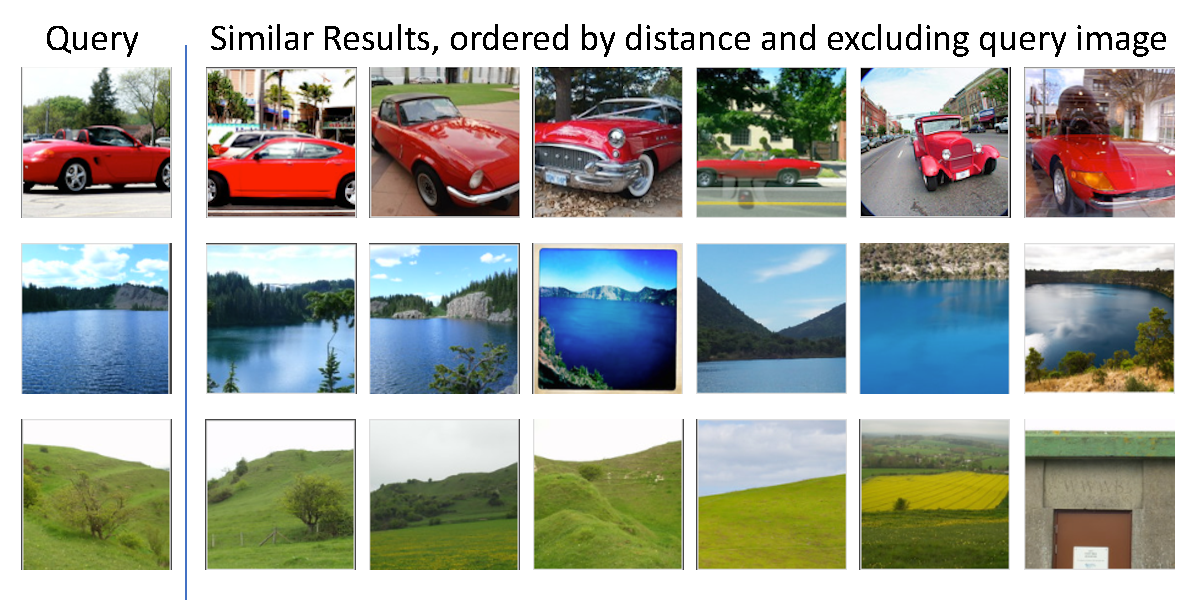
\includegraphics[width=\textwidth]{figures/feature_img_results}
\caption{Sample Results of Similarity Search}
\label{fig:similarity}
\end{figure*}

Figure \ref{fig:similarity} shows 3 examples of a query image (on the left),
and images returned as "similar" by VDMS.
The query input is a descriptor generated after a query image. The "query"
descriptor is sent to VDMS as part of the query, and VDMS use that descriptor
to find similar one, and retrieve the images associated with those "similar"
descriptors. We used this as an example and as a visual validation of the
functionality and applicability in this particular dataset, but we also
provide an analytical approach to accuracy and trade-offs in our system.
It is important to note that the accuracy of the results is entirely tied
to the quality of the descriptors chosen by the applications.
VDMS is completely agnostic to information contained within the descriptor,
and simply offers the interface to store and index them, but the quality
of the similarity result will be tied to the quality of descriptor extraction
that the application is using.


\begin{figure*}[]
\centering
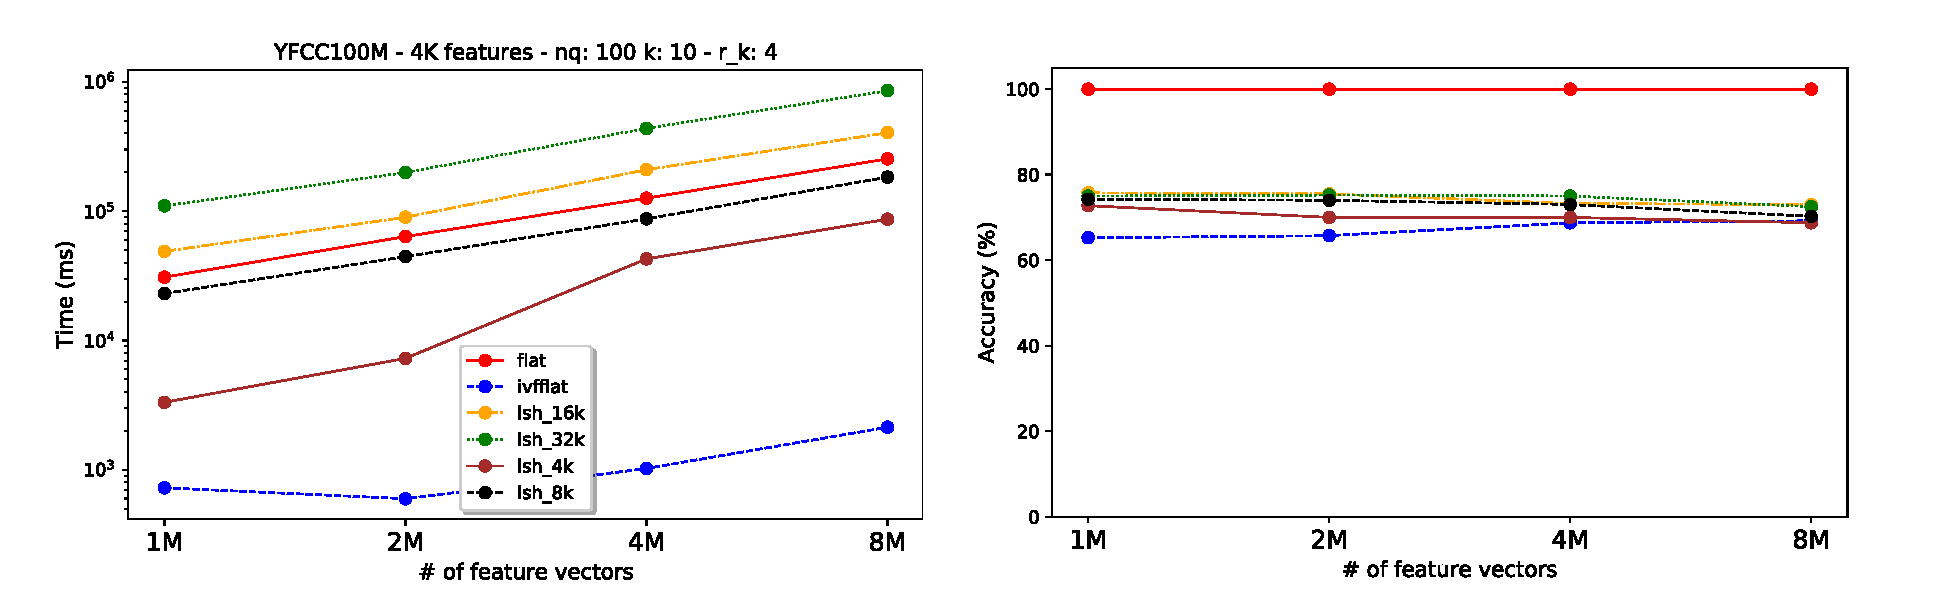
\includegraphics[width=\textwidth]{figures/features_alternatives}
\caption{Feature Vector Evaluation: Trade-off between query execution speed
and accuracy of the results, using ground-truth data for computing accuracy.
For this evaluation, we query the 10 closest neighbors (k = 10), and compute
accuracy using recall at 4 (r\_k = 4) (i.e. percentage of the top 4 ground-truth
results that is present within the top 10 computed neighbors).
We average the query execution time and accuracy for 100 queries (nq = 100).}
\label{fig:features_eval}
\end{figure*}

As mentioned before, VDMS provides different levels of customization of the
indexes created for a descriptor set, that includes the indexing techniques
and the metric for similarity.
These different indexing techniques comes with different trade-offs in terms
of speed of search and accuracy.
VDMS aims to provide functionality that is agnostics to application-specific
techniques, enabling functionality that is general to visual data processing
applications.
Figure \ref{fig:features_eval} shows an analysis at the different indexing
techniques provided by VDMS and its trade-off between accuracy and query
execution speed, for a single threaded client.
For this evaluation, we query the 10 closest neighbors (k = 10), and compute
accuracy using recall at 4 (r\_k = 4) (i.e. percentage of the top 4 ground-truth
results that is present within the top 10 computed neighbors).
We average the query execution time and accuracy for 100 queries (nq = 100).
The \textit{flat} index (red line) implements exact search and
represents ground-truth, which explain why the accuracy is always 100\% on the
right plot. The other indexes implement \textit{approximate search},
which trade-offs between accuracy and speed of search~\cite{flann, faiss}.
We have also tried the \textit{ivfflat} index (inverted file index), as well as
\textit{LSH}-based indexes using a different number of bits per descriptor
\footnote{https://github.com/facebookresearch/faiss/wiki/Faiss-indexes}.
Results show how \textit{ivfflat} is the fastest option by comes at the trade-off
of about 30\% lost in accuracy, while simple brute-force search
is among the slowest options at the expenses of 100\% accuracy,
meaning exact search.

\begin{figure*}[]
\centering
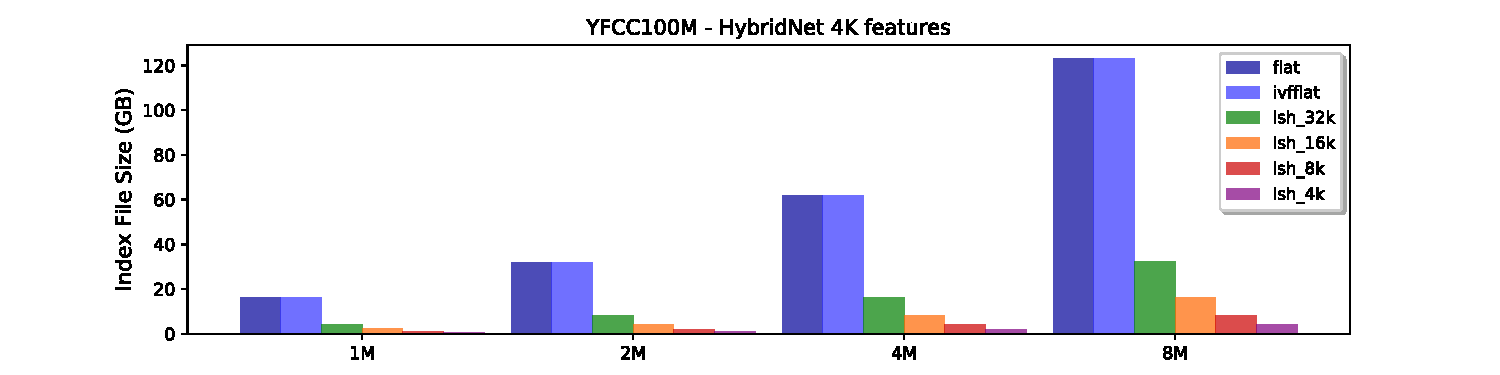
\includegraphics[width=\textwidth]{figures/features_disksize}
\caption{Feature Collection Size in Disk}
\label{fig:features_size_does_matter}
\end{figure*}

Another important trade-off to be made is w.r.t to space efficiency: Set of
descriptors can grow very large and hard to manage.
In this particular case, 4096-dimensional descriptors for 100M elements
translates into 1TB of data, only in raw floating-point data alone (without
accounting for any metadata or indexes associated with it).
This component is very important on the overall analysis because a large set
of feature vectors may not fit in memory and thus cause a pressure on the IO
system while retrieving descriptors for computing distance, that severely impact
the overall query execution time.
Because of this, when the set of descriptors grows significantly large,
it may be worth trading off accuracy to speed and space.
Figure \ref{fig:features_size_does_matter} show the different indexes and
their size in disk. These indexes already contain all the descriptors (or
a quantized version of them), and can be loaded in memory directly when it fits.
Note how, because of quantization of the descriptors, \textit{LSH} provides a
significantly lower space foot print, which can be a great option for
large collections of descriptors when accuracy is not a main factor.
